\RequirePackage{silence}
\WarningFilter{biblatex}{Patching footnotes failed}
\documentclass[10pt, compress,british,xcolor={svgnames,dvipsnames,x11names},trans]{beamer}

\usepackage{babel}
\usepackage{csquotes}
\usepackage{comment}
\usepackage{tikzsymbols}
\usepackage{colortbl}
\usepackage{xcolor}

\newcommand\Wider[2][3em]{%
\makebox[\linewidth][c]{%
  \begin{minipage}{\dimexpr\textwidth+#1\relax}
  \raggedright#2
  \end{minipage}%
  }%
}


%%% mtheme customisations
\usetheme[progressbar=frametitle,block=fill]{m}
%\setmonofont[Scale=0.92]{Fira Mono}
\AtBeginSubsection{
\metroset{color/background=dark}
\frame[plain,c]{
  \begin{center}
  \begin{minipage}{25em}
    \usebeamercolor[fg]{section title}
    \usebeamerfont{section title}
    \insertsubsection\\[-1ex]
    \usebeamertemplate*{progress bar in section page}
  \end{minipage}
  \end{center}
}
\metroset{color/background=light}
}
%%%%% end mtheme

\setbeamertemplate{frametitle continuation}[from second]
\setbeamertemplate{bibliography item}[book]

%\usepackage{xeCJK}
%\setCJKsansfont[BoldFont=Kozuka Gothic Pro]{Kozuka Gothic Pro L}
%\setCJKsansfont{IPAGothic}
% \newCJKfontfamily{\xiheifont}[BoldFont=STHeiti]{STXihei}
%\newCJKfontfamily{\xiheifont}{WenQuanYi Micro Hei}

\usetikzlibrary{arrows}
\usetikzlibrary{chains}
\usepackage{tikz-qtree}
\usepackage{multicol}


\usepackage{expex}
%\lingset{glhangindent=2em,glspace=1em,aboveexskip=0pt,belowexskip=0pt,aboveglftskip=-3pt,extraglskip=3pt} %v0.1
%\lingset{exskip=0pt,interpartskip=-3pt,belowpreambleskip=-3pt,belowglpreambleskip=-3pt,aboveglftskip=-3pt,extraglskip=3pt,glhangstyle=none}
\usepackage{relsize}
\usepackage{booktabs,tabularx}
%\usepackage{textcomp}
\usepackage{listings}

\usepackage{algorithmic}
\renewcommand{\algorithmiccomment}[1]{\alert{/* #1 */}}

\usetikzlibrary{shapes.multipart}
\usetikzlibrary{positioning}
\usetikzlibrary{arrows.meta}

\makeatletter
\pgfarrowsdeclare{crow's foot}{crow's foot}
{
  \pgfarrowsleftextend{+-.5\pgflinewidth}%
  \pgfarrowsrightextend{+.5\pgflinewidth}%
}
{
  \pgfutil@tempdima=0.5pt%
  \advance\pgfutil@tempdima by.25\pgflinewidth%
  \pgfsetdash{}{+0pt}%
  \pgfsetmiterjoin%
  \pgfpathmoveto{\pgfqpoint{0pt}{-6\pgfutil@tempdima}}%
  \pgfpathlineto{\pgfqpoint{-6\pgfutil@tempdima}{0pt}}%
  \pgfpathlineto{\pgfqpoint{0pt}{6\pgfutil@tempdima}}%
  \pgfusepathqstroke%
}

\usepackage[backend=biber,style=apa]{biblatex}
\DeclareLanguageMapping{british}{british-apa}
\renewcommand{\finalnamedelim}{and}
\renewcommand{\bibfont}{\small}
\setlength{\bibhang}{1em}
\setlength{\bibitemsep}{1ex}
\bibliography{refs}
\renewcommand{\UrlFont}{\ttfamily}

\usepackage[os=win]{menukeys}
\usepackage{caption}
\usepackage{tikz}
\usepackage{subfig}
\usepackage{amsmath}
\usepackage{amsfonts}
\usepackage{amssymb}
\usepackage{tkz-euclide}
\usepackage{graphicx}
\usepackage{graphics}
\usepackage{tikz-qtree}

\usepackage{latexsym}
\newcommand{\norm}[1]{\left\lVert#1\right\rVert}
% Following three lines are needed for this document.
% If you are not loading colors or url, then these are
% not required.
\usepackage{tabu}

\usepackage{blindtext}
\usepackage{mathtools}
\usepackage{booktabs,caption,fixltx2e}
\usepackage[flushleft]{threeparttable}
\usepackage{tabularx}
\usepackage{adjustbox}
\usepackage{soul}

\usetkzobj{all}
%usepackage{ftnxtra}
%usepackage{fnpos}
\usetikzlibrary{calc,positioning,intersections,quotes,decorations.markings,trees}

\newenvironment{figure*}%
{\begin{figure}}
{\end{figure}}

\title{Smart Room Gesture Control using Kinect skeletal data}

%\subtitle{Building the Aigaio NUI}
\subtitle{Diploma Thesis Presentation}

\date{10 July 2016}
\author{Giwrgos Paraskevopoulos}
\institute{
School of Electrical and Computer Engineering\\
National Technical University of Athens\\[2ex]
Institute of Informatics and Telecommunications\\
NCSR Demokritos
}

\institute{

\begin{columns}[T]
\begin{column}{.5\linewidth}
\begin{figure}[H]
\resizebox{.3\linewidth}{!}{

\includegraphics[]{figs/pyrforos}
}
\end{figure}
\begin{center}
School of Electrical and Computer Engineering\\
\footnotesize National Technical University of Athens
\end{center}
\end{column}

\pause

\begin{column}{=.5\linewidth}
\begin{figure}[H]
\resizebox{.28\linewidth}{!}{

\includegraphics[]{figs/demokritos}
}
\end{figure}
\begin{center}
Institute of Informatics and Telecommunications\\
\footnotesize NCSR Demokritos
\end{center}

\end{column}
\end{columns}
}

\begin{document}

\maketitle

\begin{frame}[label=LO]
\frametitle{Goals of this work}

\begin{itemize}
\item Build a simple and intuitive \textbf{Natural User Interface} for a smart conference room.
\item Use the Kinect skeletal information to devise some novel and \textbf{accurate} techniques for \textbf{pose} and \textbf{gesture} recognition focused on \textbf{real-time} systems.
\item Create efficient implementations of the devised algorithms as \textbf{microservices}.
\item Demonstrate how \textbf{Machine to Machine} communication can be used to compose these microservices into non trivial applications for the \textbf{Internet of Things} ecosystem.
\item  Integrate our work into the \textbf{Synaisthisi} platform.
\end{itemize}
\end{frame}


\begin{frame}{movie}
\frametitle{Demo Time}
\Large \href{https://www.youtube.com/watch?v=5C_p7MHKA4g}{Demo Link}
\end{frame}

\begin{frame}{Contents}
\setbeamertemplate{section in toc}[sections numbered]
\tableofcontents[hideallsubsections]
\end{frame}

%% %!TEX root = main.tex
\subsection{The Internet of Things}


\begin{frame}
\frametitle{IoT definition}
The Internet of Things is <insert preferred definition>.
\end{frame}


\begin{frame}
\frametitle{IoT definition}
The Internet of Things is a generalization of the World Wide Web to incorporate ``things'' that exist in the physical world. 
\end{frame}

\begin{frame}
\frametitle{IoT definition}
The Internet of Things is the convergence of all virtual and physical entities that are able to produce, consume and act upon data under a common communications infrastructure.
\end{frame}

\begin{frame}
\frametitle{Synaisthisi Platform}
The Synaisthisi platform is a project developed in NCSR Demokritos that aims to facilitate the development of Internet of Things applications.

It provides
\begin{itemize}
\item A \textbf{Service Oriented Architecture} where applications can be developed as the composition of small functional building blocks (services) 
\item A categorization of services in Sensing, Processing and Actuating (\textbf{SPA services})
\item A \textbf{Message Oriented Middleware} that provides a pub/sub message passing infrastructure based on MQTT for inter-service communication
\item Mechanisms for logging, security, persistent storage, data replication and administration of the applications and the system
\end{itemize}
\end{frame}


\begin{frame}
\frametitle{Synaisthisi Architecture}

\begin{figure}[!htb]
\centering
\resizebox{0.85\linewidth}{!}{
	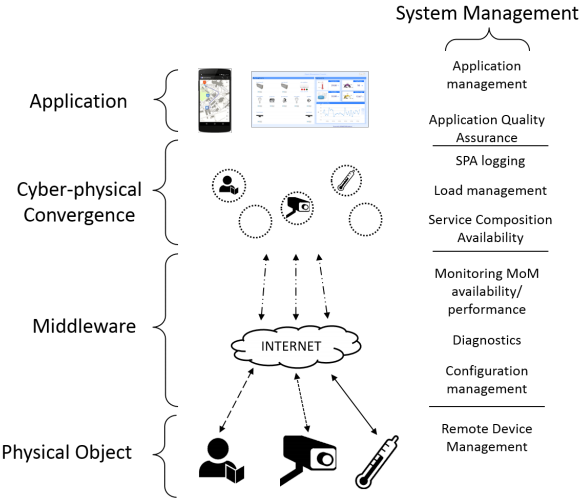
\includegraphics[]{figs/synaisthisi-arch}
}
\end{figure}

\end{frame}
%% %!TEX root = main.tex
\subsection{Machine to Machine Communication}


\begin{frame}
\frametitle{Publish/Subscribe Protocols}
Pros:

\begin{itemize}
\item Asynchronous communication
\item Decoupling of the communicating entities
\item Many to many
\item Scalable
\end{itemize}

Cons:
\begin{itemize}
\item Semantic coupling (message type needs to be statically defined)
\item Loose message delivery guarantees
\end{itemize}

\end{frame}


\begin{frame}
\frametitle{MQTT}

All of the above plus
\begin{itemize}
\item Lightweight
\item Small code footprint
\item Small header overhead
\item QoS Levels
\end{itemize}

\begin{figure}[!htb]
\centering
\resizebox{0.85\linewidth}{!}{
	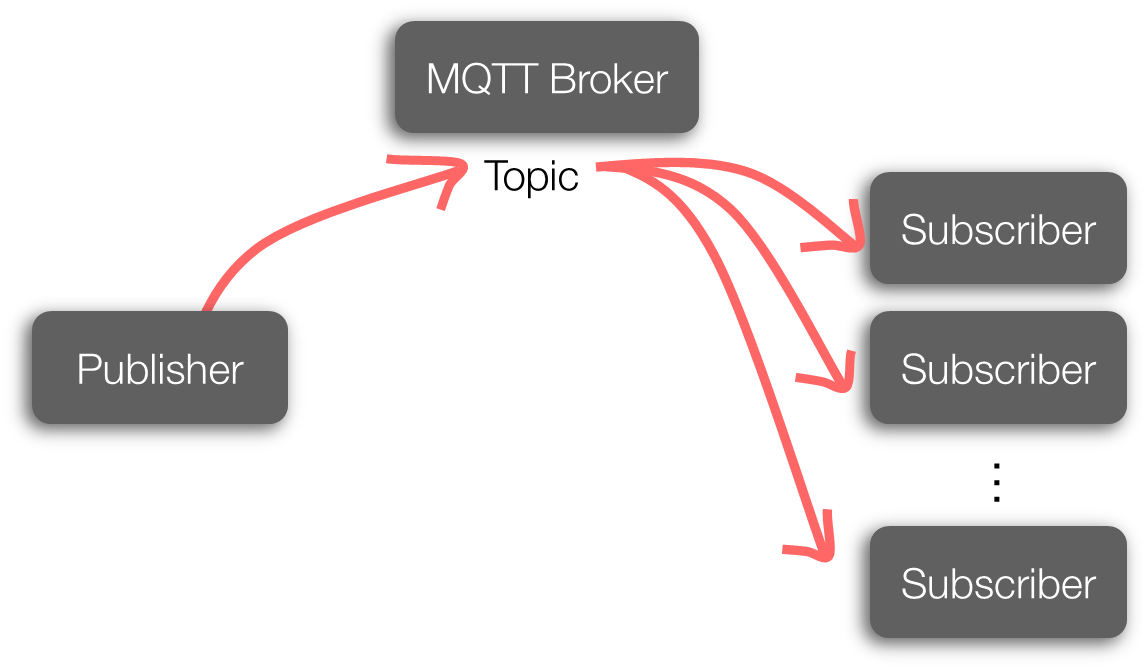
\includegraphics[]{figs/mqtt-block-diagram}
}
\end{figure}

\end{frame}

%% %!TEX root = main.tex
\subsection{The Microsoft Kinect SDK}


\begin{frame}
\frametitle{Data streams}

\begin{figure*}[ht!]
  \centering
  \begin{minipage}{0.32\textwidth}
  	\centering
    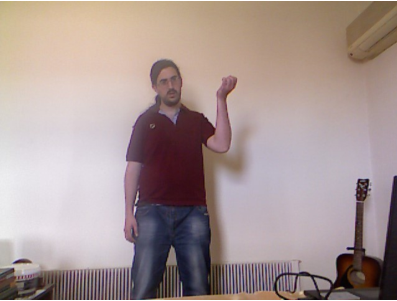
\includegraphics[width=\textwidth]{figs/color-frame}\\
    Color Stream
  \end{minipage}\hfill
  \begin{minipage}{0.32\textwidth}
  	\centering
	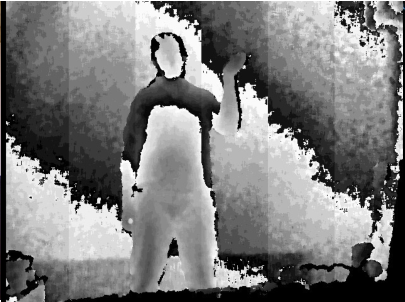
\includegraphics[width=\textwidth]{figs/depth-frame}\\
    Depth Stream
  \end{minipage}\hfill
  \begin{minipage}{0.32\textwidth}
  	\centering
    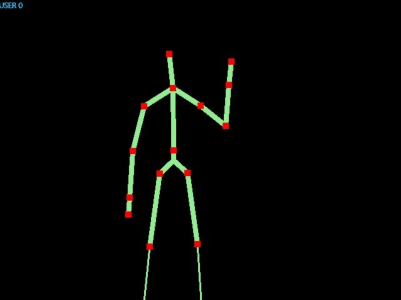
\includegraphics[width=\textwidth]{figs/skeleton-frame}\\
    Skeleton Stream
  \end{minipage}
\end{figure*}

\end{frame}


\begin{frame}
\frametitle{Skeleton Joints}
\begin{itemize}
\item A total of 20 inferred joints
\item Organized in a hierarchical structure (we make use of this later)
\end{itemize}

\begin{figure*}[ht!]
\label{fig1}
\centering
\begin{minipage}{0.34\linewidth}
\centering
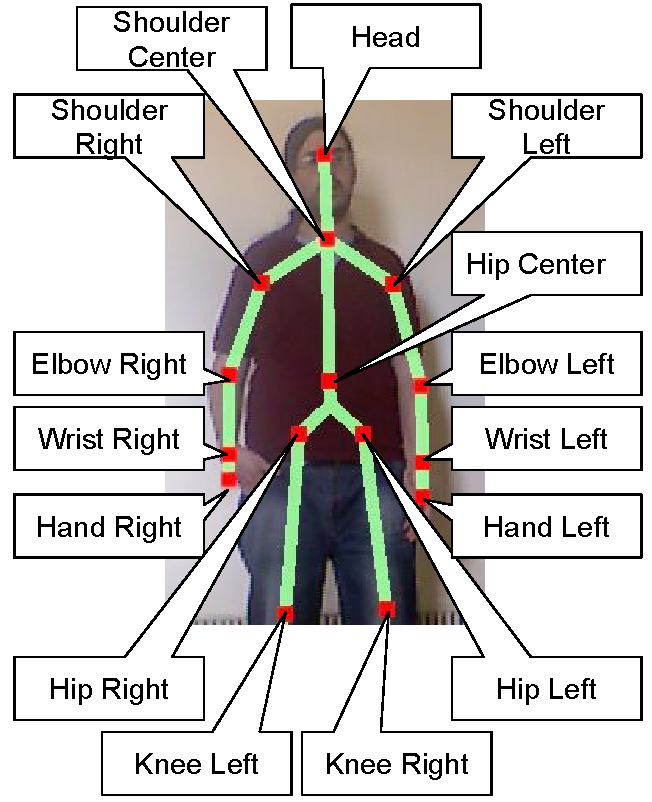
\includegraphics[width=\linewidth]{figs/skeleton.pdf}\\
Skeletal Joints
\end{minipage}\hfill
\begin{minipage}{0.6\linewidth}
\centering
\resizebox{\linewidth}{!} {
\tikzset{edge from parent/.style=
{draw, edge from parent path={(\tikzparentnode.south)
-- +(0,-3pt)
-| (\tikzchildnode)}},
blank/.style={draw=none}}
    \begin{tikzpicture}

    \node{\Tree 
     [.{HipCenter} 
        [.Spine [.{Shoulder Center}  [.{Shoulder Left} [.{Elbow Left} [.{Wrist Left} [.{Hand Left} ]]]]  {Head} [.{Shoulder Right} [.{Elbow Right} [.{Wrist Right} [.{Hand Right} ]]]]  ]]
        [.{Hip Left} [.{Knee Left} [.{Ankle Left} [.{Foot Left} ]]]]
        [.{Hip Right} [.{Knee Right} [.{Ankle Right} [.{Foo tRight} ]]]]
        ]};
    \end{tikzpicture}
}\\
Joints in a tree structure
\end{minipage}

\end{figure*}
\end{frame}

%!TEX root = main.tex
\section{Pose Detection}


\begin{frame}
\frametitle{Problem Definition}

\begin{itemize}
\item A pose is the temporary suspension of the animation of the body joints in a discrete configuration.
\item Pose detection is the problem of automatically classifying a pose.
\item \textit{Poses can be used as control signals}
\end{itemize}
\end{frame}


\begin{frame}
\frametitle{Assumptions}

\begin{itemize}
\item Sufficient room \textbf{lighting} conditions for the operation of the Kinect sensor
\item User is positioned \textbf{inside the operating area} of the Kinect sensor and is \textbf{facing} the sensor
\item \textbf{Predefined} set of target poses
\end{itemize}

\end{frame}

\begin{frame}
\frametitle{Design Prerequisites}

Detection is

\begin{itemize}
\item \textbf{real-time}
\item invariant to the user \textbf{position} and \textbf{distance} from the camera
\item invariant to the user \textbf{physical characteristics} (height, weight etc.)
\item able to support \textbf{multiple users} (a limit of 2 is imposed by the Kinect sensor)
\end{itemize}

\end{frame}

\begin{frame}
\frametitle{The proposed algorithm}

\begin{itemize}
\item Template matching to a set of geometric features
\item Poses are predefined templates
\item We compare the current feature vector to the template, and if it is within a predefined error margin the pose is recognized
\end{itemize}

\begin{center}
\textbf{Simple, fast and performs well in real world scenarios.}
\end{center}

\end{frame}

% %!TEX root = main.tex
\subsection{The Microsoft Kinect SDK}


\begin{frame}
\frametitle{Data streams}

\begin{figure*}[ht!]
  \centering
  \begin{minipage}{0.32\textwidth}
  	\centering
    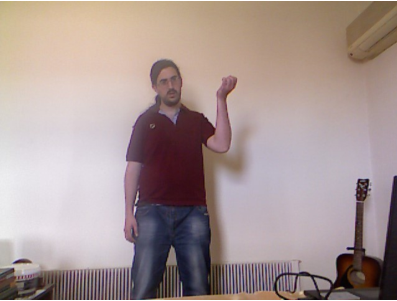
\includegraphics[width=\textwidth]{figs/color-frame}\\
    Color Stream
  \end{minipage}\hfill
  \begin{minipage}{0.32\textwidth}
  	\centering
	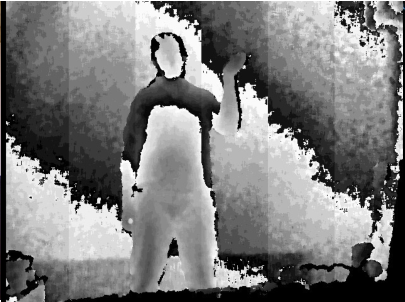
\includegraphics[width=\textwidth]{figs/depth-frame}\\
    Depth Stream
  \end{minipage}\hfill
  \begin{minipage}{0.32\textwidth}
  	\centering
    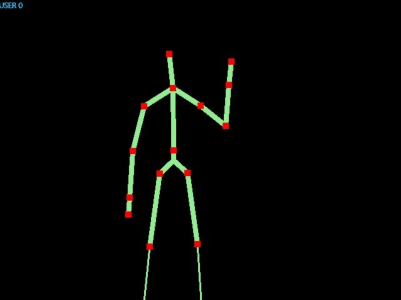
\includegraphics[width=\textwidth]{figs/skeleton-frame}\\
    Skeleton Stream
  \end{minipage}
\end{figure*}

\end{frame}


\begin{frame}
\frametitle{Skeleton Joints}
\begin{itemize}
\item A total of 20 inferred joints
\item Organized in a hierarchical structure (we make use of this later)
\end{itemize}

\begin{figure*}[ht!]
\label{fig1}
\centering
\begin{minipage}{0.34\linewidth}
\centering
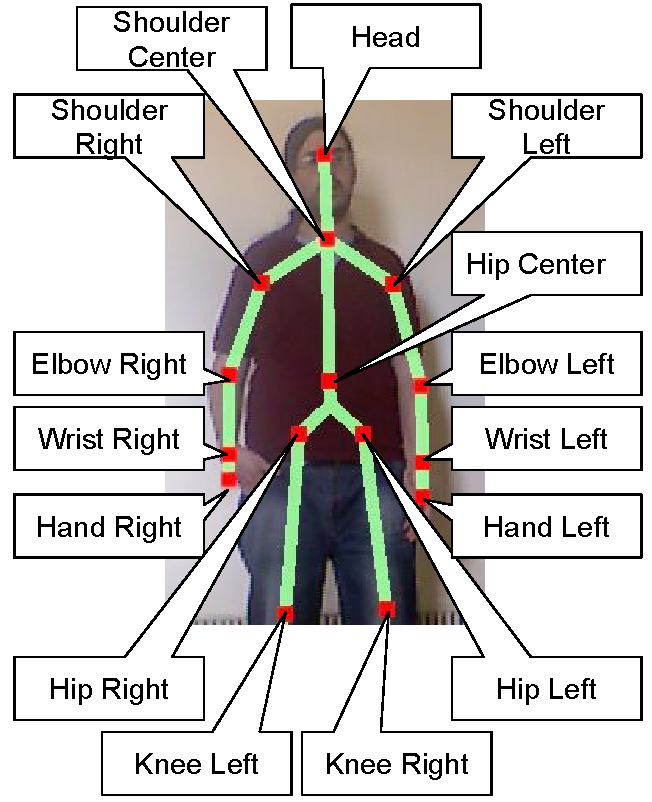
\includegraphics[width=\linewidth]{figs/skeleton.pdf}\\
Skeletal Joints
\end{minipage}\hfill
\begin{minipage}{0.6\linewidth}
\centering
\resizebox{\linewidth}{!} {
\tikzset{edge from parent/.style=
{draw, edge from parent path={(\tikzparentnode.south)
-- +(0,-3pt)
-| (\tikzchildnode)}},
blank/.style={draw=none}}
    \begin{tikzpicture}

    \node{\Tree 
     [.{HipCenter} 
        [.Spine [.{Shoulder Center}  [.{Shoulder Left} [.{Elbow Left} [.{Wrist Left} [.{Hand Left} ]]]]  {Head} [.{Shoulder Right} [.{Elbow Right} [.{Wrist Right} [.{Hand Right} ]]]]  ]]
        [.{Hip Left} [.{Knee Left} [.{Ankle Left} [.{Foot Left} ]]]]
        [.{Hip Right} [.{Knee Right} [.{Ankle Right} [.{Foo tRight} ]]]]
        ]};
    \end{tikzpicture}
}\\
Joints in a tree structure
\end{minipage}

\end{figure*}
\end{frame}


\subsection{The Algorithm}

\begin{frame}
\frametitle{Geometric Features}

\begin{itemize}
\item Make use of the joints \textbf{hierarchical} structure to compute the \textbf{angles between} each \textbf{parent} and \textbf{child} joint.

\item This \textbf{single} feature provides by default the \textbf{position} and \textbf{depth invariance} and is \textbf{enough} to classify a \textbf{large set} of poses.
\end{itemize}
\end{frame}

\begin{frame}
\frametitle{Feature Calculation}


\begin{figure}[!htb]
\centering
\resizebox{0.3\linewidth}{!} {
  \begin{tikzpicture}[scale=1]
     \coordinate (A) at (2,5);
     \coordinate (B) at (6,3); 
     \coordinate (C) at (2,0);
     \draw (A) -- (B) node [anchor=south]{$B$} node [midway, above] {$c$};
     \draw (B) -- (C) node [anchor=north]{$C$} node [midway, right] {$a$};
     \draw (C) -- (A) node [anchor=south]{$A$} node [midway, left] {$b$};
     \tkzMarkAngle(B,C,A);
   \end{tikzpicture}
}\\
\small The triangle that is formed between the father joint $A$, the child joint $B$ and the point $(A.x, 0)$
 \end{figure}

Using the law of cosines, we calculate the $\angle{ACB}$ as

\begin{equation}
C=\cos^{-1}\frac{a^2+b^2-c^2}{2ab}
\end{equation}

\end{frame}

\begin{frame}[fragile]
\frametitle{Example Pose Template}

\begin{columns}[T]
\begin{column}{.5\linewidth}

\begin{figure}[!ht]
\centering
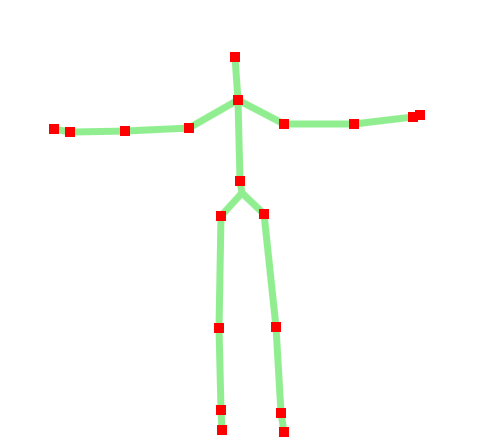
\includegraphics[width=\linewidth]{figs/hands-apart-pose.png}
\end{figure}

\end{column}

\pause

\begin{column}{.5\linewidth}

\begin{minipage}{\linewidth}

\lstset{
   basicstyle=\ttfamily,
   columns=fullflexible,
   showstringspaces=false%,
%   commentstyle=\color{gray}\upshape
 }

\begin{lstlisting}[
    basicstyle=\tiny, %or \small or \footnotesize etc.
]
 <?xml version="1.0" encoding="utf-8" ?>
 <Pose id="HANDSAPART"
       xmlns:xsi="http://www.w3.org/2001/XMLSchema-instance"
       xsi:schemaLocation="urn:PoseRules PoseRules.xsd">
     <DisplayName>Jack I'm Flying</DisplayName>
     <AngleConstraints units="degrees">
         <ElbowLeft>
             <Desired>180</Desired>
             <Deviation>15</Deviation>
         </ElbowLeft>
         <HandLeft>
             <Desired>180</Desired>
             <Deviation>15</Deviation>
         </HandLeft>
         <ElbowRight>
             <Desired>0</Desired>
             <Deviation>15</Deviation>
         </ElbowRight>
         <HandRight>
             <Desired>0</Desired>
             <Deviation>15</Deviation>
         </HandRight>
     </AngleConstraints>
 </Pose>
 \end{lstlisting}
\end{minipage}
\end{column}

\end{columns}

\end{frame}

%!TEX root = main.tex
\section{Gesture Recognition}

\begin{frame}
\frametitle{What is a gesture?}

\begin{itemize}
\item A continuous stream of poses
\item The transfer of a subset of joints from point A to B, using a vaguely predefined trajectory
\end{itemize}
\end{frame}

\begin{frame}
\frametitle{What is a gesture?}
\begin{itemize}
\item \st{A continuous stream of poses}
\item \textbf{The transfer of a subset of joints from point A to B, using a vaguely predefined trajectory}
\end{itemize}

\end{frame}

\begin{frame}
\frametitle{Gesture Example}

\begin{center}
Swipe In (Right Hand)

\begin{figure}[!htb]
\centering
\resizebox{\linewidth}{!}{
	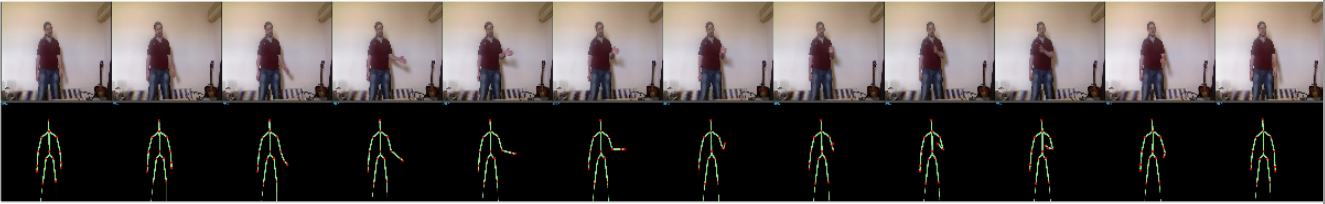
\includegraphics[]{figs/swipein-frameseq}
}
\end{figure}


\end{center}

\begin{center}
Swipe Up (Right Hand)

\begin{figure}[!htb]
\centering
\resizebox{\linewidth}{!}{
	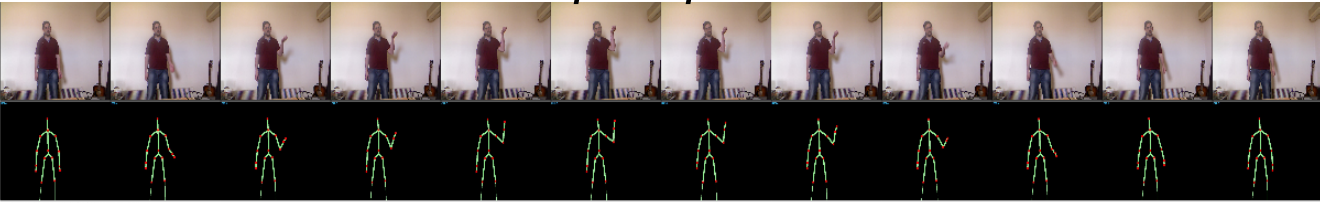
\includegraphics[]{figs/swipeup-frameseq}
}
\end{figure}


\end{center}
\end{frame}



\begin{frame}
\frametitle{The proposed approach}

\begin{itemize}
\item Extract a set of \textbf{low level geometric} features
\item Evaluate the performance (classification \textbf{accuracy} and \textbf{time}) of a set of well known machine learning techniques on this set of features
\end{itemize}

\end{frame}

\subsection{Feature Extraction}

\begin{frame}
\frametitle{Feature Extraction}

\begin{itemize}
\item We are interested in gestures; use only elbows, wrists and hands (LeftElbow, RightElbow, LeftWrist, RightWrist, LeftHand, RightHand)
\item For each we calculate a set of features, for the set of N frames that correspond to the gesture and based on their 3D coordinates
\end{itemize}

\end{frame}

\begin{frame}
\frametitle{Feature Properties}

Our features satisfy the following

\begin{itemize}
\item They require constant time \textbf{O(1)} in each frame to compute
\item Small gesture changes are reflected to small feature changes (angle and displacement are able to \textbf{discriminate between small movements})
\item They are aggregate features that \textbf{summarize} the gesture over all the frames
\item They are \textbf{small in size} (a feature vector in minified JSON format is about 3KB)
\end{itemize}

\end{frame}

\begin{frame}
\frametitle{The Features}

\begin{columns}[T]

\begin{column}{.4\linewidth}
Features are extracted
\begin{itemize}
\item from each skeletal \textbf{joint}
\item from a set of the \textbf{frames} depicting the gesture
\item using the \textbf{3D coordinates} of the joints
\end{itemize}

\end{column}

\pause

\begin{column}{.7\linewidth}
\resizebox{\linewidth}{!}{

    \begin{tabular}{|c|c|c|}
        \hline
         \textbf{Feature name}  & \textbf{Frames involved}  & \textbf{Equation}  \\ \hline
         Spatial angle          & $F_2, F_1$                  & $\displaystyle \frac{\mathbf{v}^{(J)}_{2} - \mathbf{v}^{(J)}_{1}}{\left\lVert \mathbf{v}^{(J)}_{2} - \mathbf{v}^{(J)}_{1} \right\rVert}$\\ \hline
         Spatial angle          & $F_n, F_{n-1}$              & $\displaystyle \frac{\mathbf{v}^{(J)}_{n} - \mathbf{v}^{(J)}_{n-1}}{\left\lVert \mathbf{v}^{(J)}_{n} - \mathbf{v}^{(J)}_{n-1} \right\rVert}$\\ \hline
         Spatial angle          & $F_n, F_{1}$              & $\displaystyle \frac{\mathbf{v}^{(J)}_{n} - \mathbf{v}^{(J)}_{1}}{\left\lVert \mathbf{v}^{(J)}_{n} - \mathbf{v}^{(J)}_{1} \right\rVert}$\\ \hline
         Total vector angle     & $F_1,\ldots, F_n$         & $\displaystyle \sum_{i=1}^n\arccos \left(\frac{\mathbf{v}^{(J)}_{i} \cdot \mathbf{v}^{(J)}_{i-1}}{\left\lVert \mathbf{v}^{(J)}_{i} \right\rVert \left\lVert \mathbf{v}^{(J)}_{i-1} \right\rVert}\right)$ \\ \hline
         Squared total vector angle     & $F_1,\ldots, F_n$         & $\displaystyle \sum_{i=1}^n\arccos \left(\frac{\mathbf{v}^{(J)}_{i} \cdot \mathbf{v}^{(J)}_{i-1}}{\left\lVert \mathbf{v}^{(J)}_{i} \right\rVert \left\lVert \mathbf{v}^{(J)}_{i-1} \right\rVert}\right)^2$ \\ \hline
         Total vector displacement      & $F_n, F_1$                &$\displaystyle \mathbf{v}^{(J)}_{n}-\mathbf{v}^{(J)}_{1}$ \\ \hline
         Total displacement             & $F_1,\ldots, F_n$         & $\displaystyle \sum_{i=1}^n{\mathbf{v}^{(J)}_{i} - \mathbf{v}^{(J)}_{i-1}}$ \\ \hline
         Maximum displacement & $F_1,\ldots, F_n$ & $\displaystyle \max_n\left(\mathbf{v}^{(J)}_{i}-\mathbf{v}^{(J)}_{i-1} \right)$ \\ \hline
         Bounding box diagonal length{$^*$}          & $F_1,\ldots, F_n$                  & $\displaystyle \sqrt{a_{B(\mathcal{V^{(J)}})}^2+b_{B(\mathcal{V^{(J)}})}^2}$\\ \hline
         Bounding box angle{$^*$}                 & $F_1,\ldots, F_n$                     & $\displaystyle \arctan{\frac{b_{B(\mathcal{V^{(J)}})}}{a_{B(\mathcal{V^{(J)}})}}}$ \\ \hline
    \end{tabular}
% }
%    }
}
\end{column}

\end{columns}

\end{frame}


\begin{frame}
\frametitle{The Features (cont'd)}
We also extract the initial and final (i.e., at $F_1$ and $F_N$, respectively), mean and maximum \textbf{angle} (i.e., for $F_1,\ldots F_N$) between any pair of joints (pc = parent-child )

\begin{equation} \label{eq:1}
\theta_{pc} = \cos^{-1}\left(\frac{a_{pc}^2+b_{pc}^2-c_{pc}^2}{2a_{pc}b_{pc}}\right)
\end{equation}

\noindent where

\begin{equation}
a_{pc} = \left(v^{(J)}_χ - v^{(J_c)}_x\right)^2 + \left(v^{(J)}_y - v^{(J_c)}_y\right)^2  \ ,
\end{equation}
\begin{equation}
b_{pc} = v^{(J)}_x \ \text{και}
\end{equation}
\begin{equation}
c_{pc} = (v^{(J_p)}_x)^2 + (v^{(J)}_y - v^{(J_p)}_y)^2  \ .
\end{equation}

\end{frame}

\begin{frame}
\frametitle{The Features (cont'd)}
Finally between HandLeft and HandRight and within the gesture we extract

\begin{itemize}
\item The max...
\begin{equation}
\label{eq:maxd}
d_{\text{max}}=\max_{i,j} \left \{d\left(\mathbf{v}_i^{\text{HR}},\mathbf{v}_j^{\text{HL}}\right) \right \} \ ,
\end{equation}
\item ... and the mean distance
\begin{equation}
\label{eq:meand}   
d_{\text{mean}}= \frac{1}{F^{(J)}} \sum_{i,j} d\left(\mathbf{v}_i^{\text{HR}},\mathbf{v}_j^{\text{HL}}\right) \ ,
\end{equation}
\end{itemize}

\end{frame}

\subsection{Experiments}

\begin{frame}
\frametitle{Machine Learning approaches}

For gesture recognition based on the aforementioned features,
we investigated the following techniques:
\begin{itemize}
\item SVM Linear/RBF kernel (LSVM/RBFSVM)
\item Linear Discriminant Analysis (LDA)
\item Quadratic Discriminant Analysis (QDA)
\item Naive Bayes (NB)
\item K-nearest neighbors (KNN)
\item Decision Trees (DT)
\item Random Forests (RF)
\item Extra Trees (ET)
\item Adaboost with Decision Trees / Extra Trees (ABDT/ABET)
\end{itemize}

\end{frame}


\begin{frame}
\frametitle{Experiments Preparation - Dataset Construction}
\begin{itemize}
\item We constructed a real-life data set of \textbf{10 users} (7M/3F), ages: 22–36
\item We selected a set of “swipes” (in/out/up/down) for both hands (\textbf{8 gestures})
\item Each user performed a gesture at least \textbf{10 times}
\item We manually \textbf{``cleaned''} the dataset from obviously ``wrongly'' performed gestures
\item Each user was equipped with a \textbf{push button}, used to signify the beginning/ending of a gesture
\end{itemize}
\end{frame}


\begin{frame}
\frametitle{Experiments Preparation - Optimal Parameters}

Find the optimal parameter set for each algorithm using \textbf{Exhaustive Grid Search}

\begin{table}[htb]
\centering
\resizebox{.7\columnwidth}{!}{%
    \begin{tabular}{l l | l l}
        $\alpha$    & learning rate                 & $n$ & number of neighbors \\
        $e$         & number of estimators          & $s$ & search algorithm \\
        $d$         & maximum depth                 & $m$ & metric between point $p$ and $q$ \\
        $f$         & maximum number of features    & $r$ & regularization parameter
    \end{tabular}
}
\end{table}

\begin{table}[htb]
\centering
\resizebox{.7\columnwidth}{!}{%
\begin{tabular}{|l|l|}
\hline
Classifier   & Parameters                                                           \\ \hline
ABDT         & $e=103$, $\alpha=621.6$                                              \\ \hline
ABET         & $e=82$, $\alpha=241.6$                                               \\ \hline
DT           & $d=48$, $f=49$                                                       \\ \hline
ET           & $d=17$, $f=70$, $e=70$                                               \\ \hline
KNN          & $n=22$, $s=kd\_tree$, $m=\sum_{i=1}^{n}(\left|p_i - q_i\right|)$     \\ \hline
LSVM         & $C=0.0091$                                                           \\ \hline
QDA          & $r=0.88889$                                                          \\ \hline
RBFSVM       & $C=44.445$, $\gamma=0.0001$                                          \\ \hline
RF           & $d=27$, $f=20$, $e=75$                                               \\ \hline
\end{tabular}

}
\end{table}

\end{frame}


\begin{frame}
\frametitle{Experiment 1 - Performance for a known set of users}
\textbf{TARGET}
\begin{itemize}
\item Find the \textbf{optimal} machine learning approach to split our feature space
\end{itemize}

\textbf{METHOD}
\begin{itemize}
\item Train using gestures from all users
\item Evaluate using different gestures from all users
\item Use standard \textbf{Stratified K-fold Cross Validation}
\end{itemize}
\end{frame}


\begin{frame}
\frametitle{Experiment 1 - Results}
\Wider[5em]{
\begin{figure}[!htb]
\centering
\resizebox{\columnwidth}{!}{
	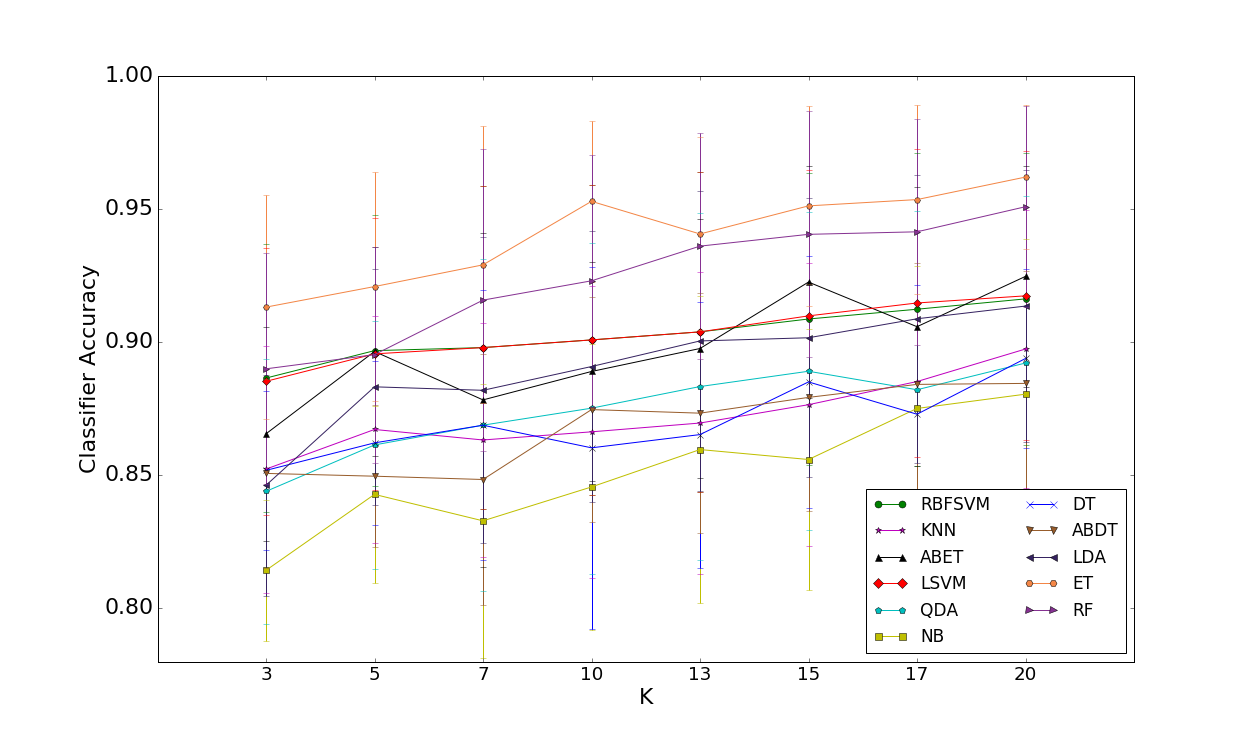
\includegraphics[]{figs/kfold}
}
\end{figure}
}
\end{frame}



\begin{frame}
\frametitle{Experiment 2 - Performance against unknown users}

\textbf{TARGET}

What is
\begin{itemize}
\item the performance for \textbf{new} / \textbf{unknown} users?
\item the \textbf{minimum} number of \textbf{users} that can be used for \textbf{training} and get an adequate classifier?
\item the effect of \textbf{``bad users''}?
\end{itemize}

\textbf{METHOD}

\begin{itemize}
\item Split the data per user
\item Use a varying number of users for training and the rest for testing
\end{itemize}

\end{frame}


\begin{frame}
\frametitle{Experiment 2 - Results per user ($F1$ score)}
\begin{table}[ht!]
\centering
\resizebox{\columnwidth}{!}{%

\begin{tabular}{l|>{\columncolor[gray]{0.9}}ccccccccccc}
\toprule
             & User 1 & User 2 & User 3 & User 4 & User 5 & User 6 & User 7 & User 8 & User 9 & User 10 & Mean w/o User 1 \\ 
\midrule
LH-SwipeDown &    0.76    &   0.83     &  1.00      &   0.82     &   1.00     &   0.80   &    1.00    &   1.00     &  1.00      &   0.96  & \textbf{0.934}    \\
LH-SwipeIn   &    0.38    &   0.92     &  0.84      &   1.00     &   1.00     &   0.92   &    1.00    &   1.00     &  1.00      &   1.00  & \textbf{0.964}    \\
LH-SwipeOut  &    0.61    &   0.93     &  0.86      &   1.00     &   1.00     &   0.89   &    1.00    &   1.00     &  0.97      &   1.00  & \textbf{0.961}    \\
LH-SwipeUp   &    0.69    &   0.90     &  1.00      &   0.84     &   1.00     &   0.83   &    1.00    &   1.00     &  0.97      &   0.96  & \textbf{0.944}    \\
RH-SwipeDown &    0.78    &   1.00     &  0.95      &    -       &   1.00     &   1.00   &    0.92    &   1.00     &  0.87      &   1.00  & \textbf{0.968}    \\
RH-SwipeIn   &    0.64    &   1.00     &  0.67      &    -       &   1.00     &   1.00   &    1.00    &   1.00     &  0.89      &   0.96  & \textbf{0.940}    \\
RH-SwipeOut  &    0.61    &   1.00     &  0.80      &    -       &   1.00     &   1.00   &    0.95    &   1.00     &  1.00      &   0.95  & \textbf{0.963}    \\
RH-SwipeUp   &    0.40    &   1.00     &  0.95      &    -       &   1.00     &   1.00   &    1.00    &   1.00     &  0.96      &   1.00  & \textbf{0.989}    \\
Average      &    \textbf{0.62}    &   \textbf{0.94}     &  \textbf{0.88}      &   \textbf{0.92}     &   \textbf{1.00}     &   \textbf{0.92}     &    \textbf{0.99}    &   \textbf{1.00}   &  \textbf{0.96}      &   \textbf{0.97}     \\
\bottomrule
\end{tabular}
}
\end{table}

\end{frame}


\begin{frame}
\frametitle{Experiment 2 - Results}
\Wider[5em]{
\begin{figure}[!htb]
\centering
\resizebox{\columnwidth}{!}{
	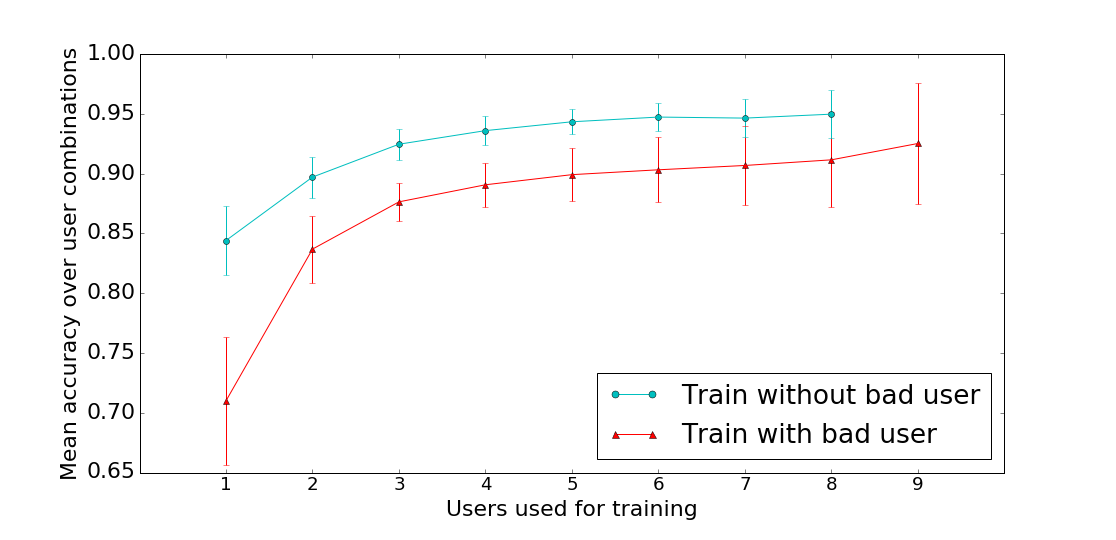
\includegraphics[]{figs/train_with_X_users}
}
\end{figure}
}
\end{frame}

\begin{frame}
\frametitle{Experiment 3 - Benchmarks}
\textbf{TARGET}
\begin{itemize}
\item Test the prediction time in different architectures
\end{itemize}

\textbf{METHOD}

Construct a custom benchmark where:
\begin{itemize}
\item \textbf{Split} the data \textbf{randomly} in train/test sets ($80$/$20$ split)
\item Classify every sample in the test data \textbf{$1000$ times}
\item Calculate the \textbf{average prediction time} for each classifier
\item Evaluate in different \textbf{architectures}
\end{itemize}

\end{frame}


\begin{frame}
\frametitle{Experiment 3 - Results}
\Wider[5em]{

\begin{figure}[!htb]
\centering
\resizebox{\columnwidth}{!}{
	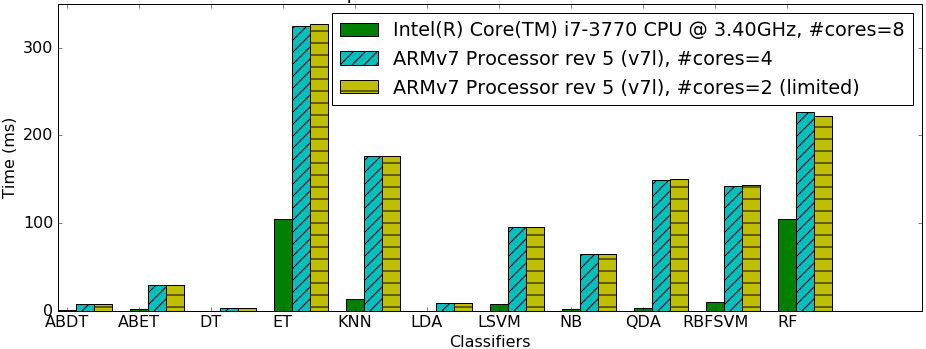
\includegraphics[]{figs/benchmark-times}
}
\end{figure}
}
\end{frame}

%!TEX root = main.tex
\section{Use Case: Smart Room Control}

\begin{frame}
\frametitle{Use Case}

The described algorithms are combined into an \textbf{IOT} application implementing a \textbf{NUI} system that is integrated into the \textbf{SYNAISTHISI} platform.

This system is used to \textbf{control the devices} inside in the \textbf{Aigaio} meeting room which is located in IIT Demokritos.

\end{frame}

% %!TEX root = main.tex
\subsection{The Internet of Things}


\begin{frame}
\frametitle{IoT definition}
The Internet of Things is <insert preferred definition>.
\end{frame}


\begin{frame}
\frametitle{IoT definition}
The Internet of Things is a generalization of the World Wide Web to incorporate ``things'' that exist in the physical world. 
\end{frame}

\begin{frame}
\frametitle{IoT definition}
The Internet of Things is the convergence of all virtual and physical entities that are able to produce, consume and act upon data under a common communications infrastructure.
\end{frame}

\begin{frame}
\frametitle{Synaisthisi Platform}
The Synaisthisi platform is a project developed in NCSR Demokritos that aims to facilitate the development of Internet of Things applications.

It provides
\begin{itemize}
\item A \textbf{Service Oriented Architecture} where applications can be developed as the composition of small functional building blocks (services) 
\item A categorization of services in Sensing, Processing and Actuating (\textbf{SPA services})
\item A \textbf{Message Oriented Middleware} that provides a pub/sub message passing infrastructure based on MQTT for inter-service communication
\item Mechanisms for logging, security, persistent storage, data replication and administration of the applications and the system
\end{itemize}
\end{frame}


\begin{frame}
\frametitle{Synaisthisi Architecture}

\begin{figure}[!htb]
\centering
\resizebox{0.85\linewidth}{!}{
	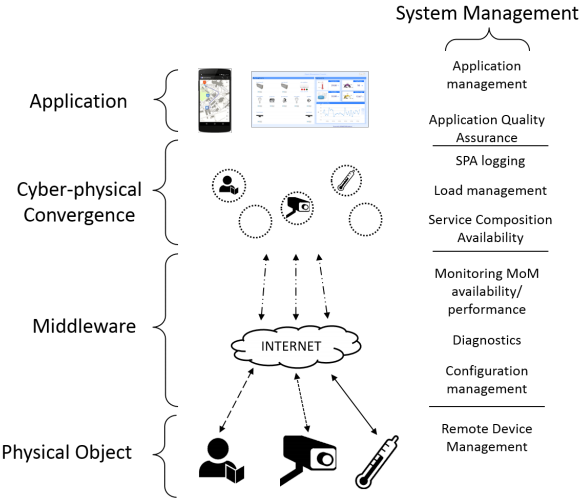
\includegraphics[]{figs/synaisthisi-arch}
}
\end{figure}

\end{frame}

% %!TEX root = main.tex
\subsection{Machine to Machine Communication}


\begin{frame}
\frametitle{Publish/Subscribe Protocols}
Pros:

\begin{itemize}
\item \textbf{Asynchronous} communication
\item \textbf{Decoupling} of the communicating entities
\item \textbf{Many to many} communication
\item \textbf{Scalable}
\end{itemize}

Cons:
\begin{itemize}
\item \textbf{Semantic coupling} (message type needs to be statically defined)
\item \textbf{Loose} message delivery \textbf{guarantees}
\end{itemize}

\end{frame}


\begin{frame}
\frametitle{MQTT}

All of the above plus
\begin{itemize}
\item Lightweight
\item Small code footprint
\item Small header overhead
\item QoS Levels
\end{itemize}

\begin{figure}[!htb]
\centering
\resizebox{0.85\linewidth}{!}{
	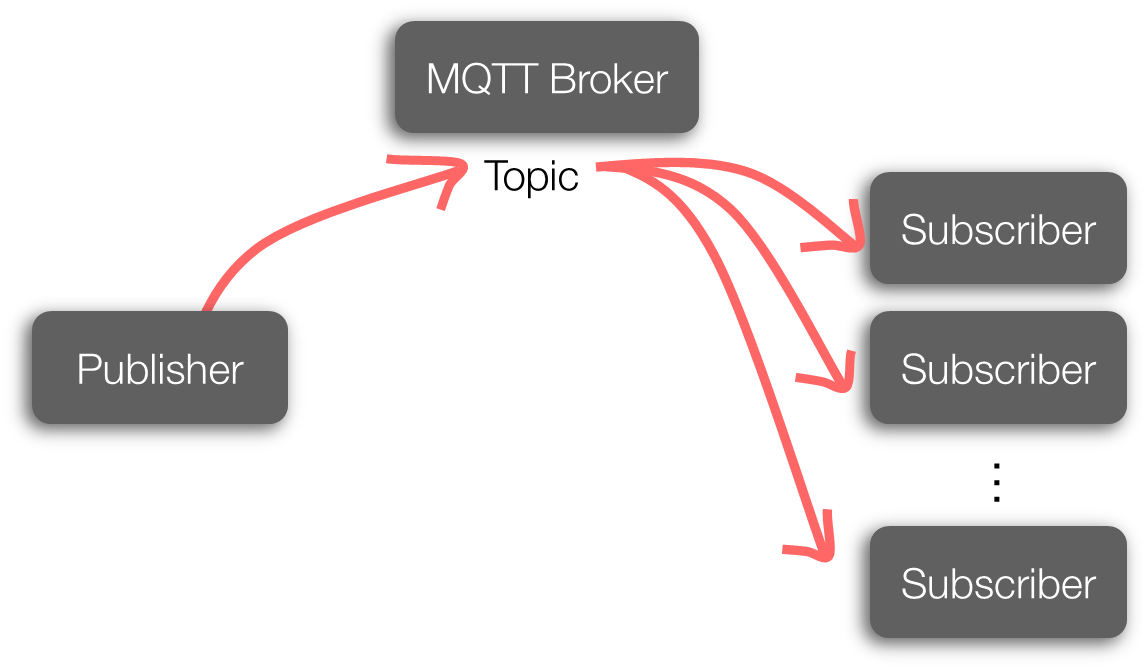
\includegraphics[]{figs/mqtt-block-diagram}
}
\end{figure}

\end{frame}


\subsection{System Design}

\begin{frame}
\frametitle{Aigaio Devices}
\Wider[1em] {
\begin{figure}
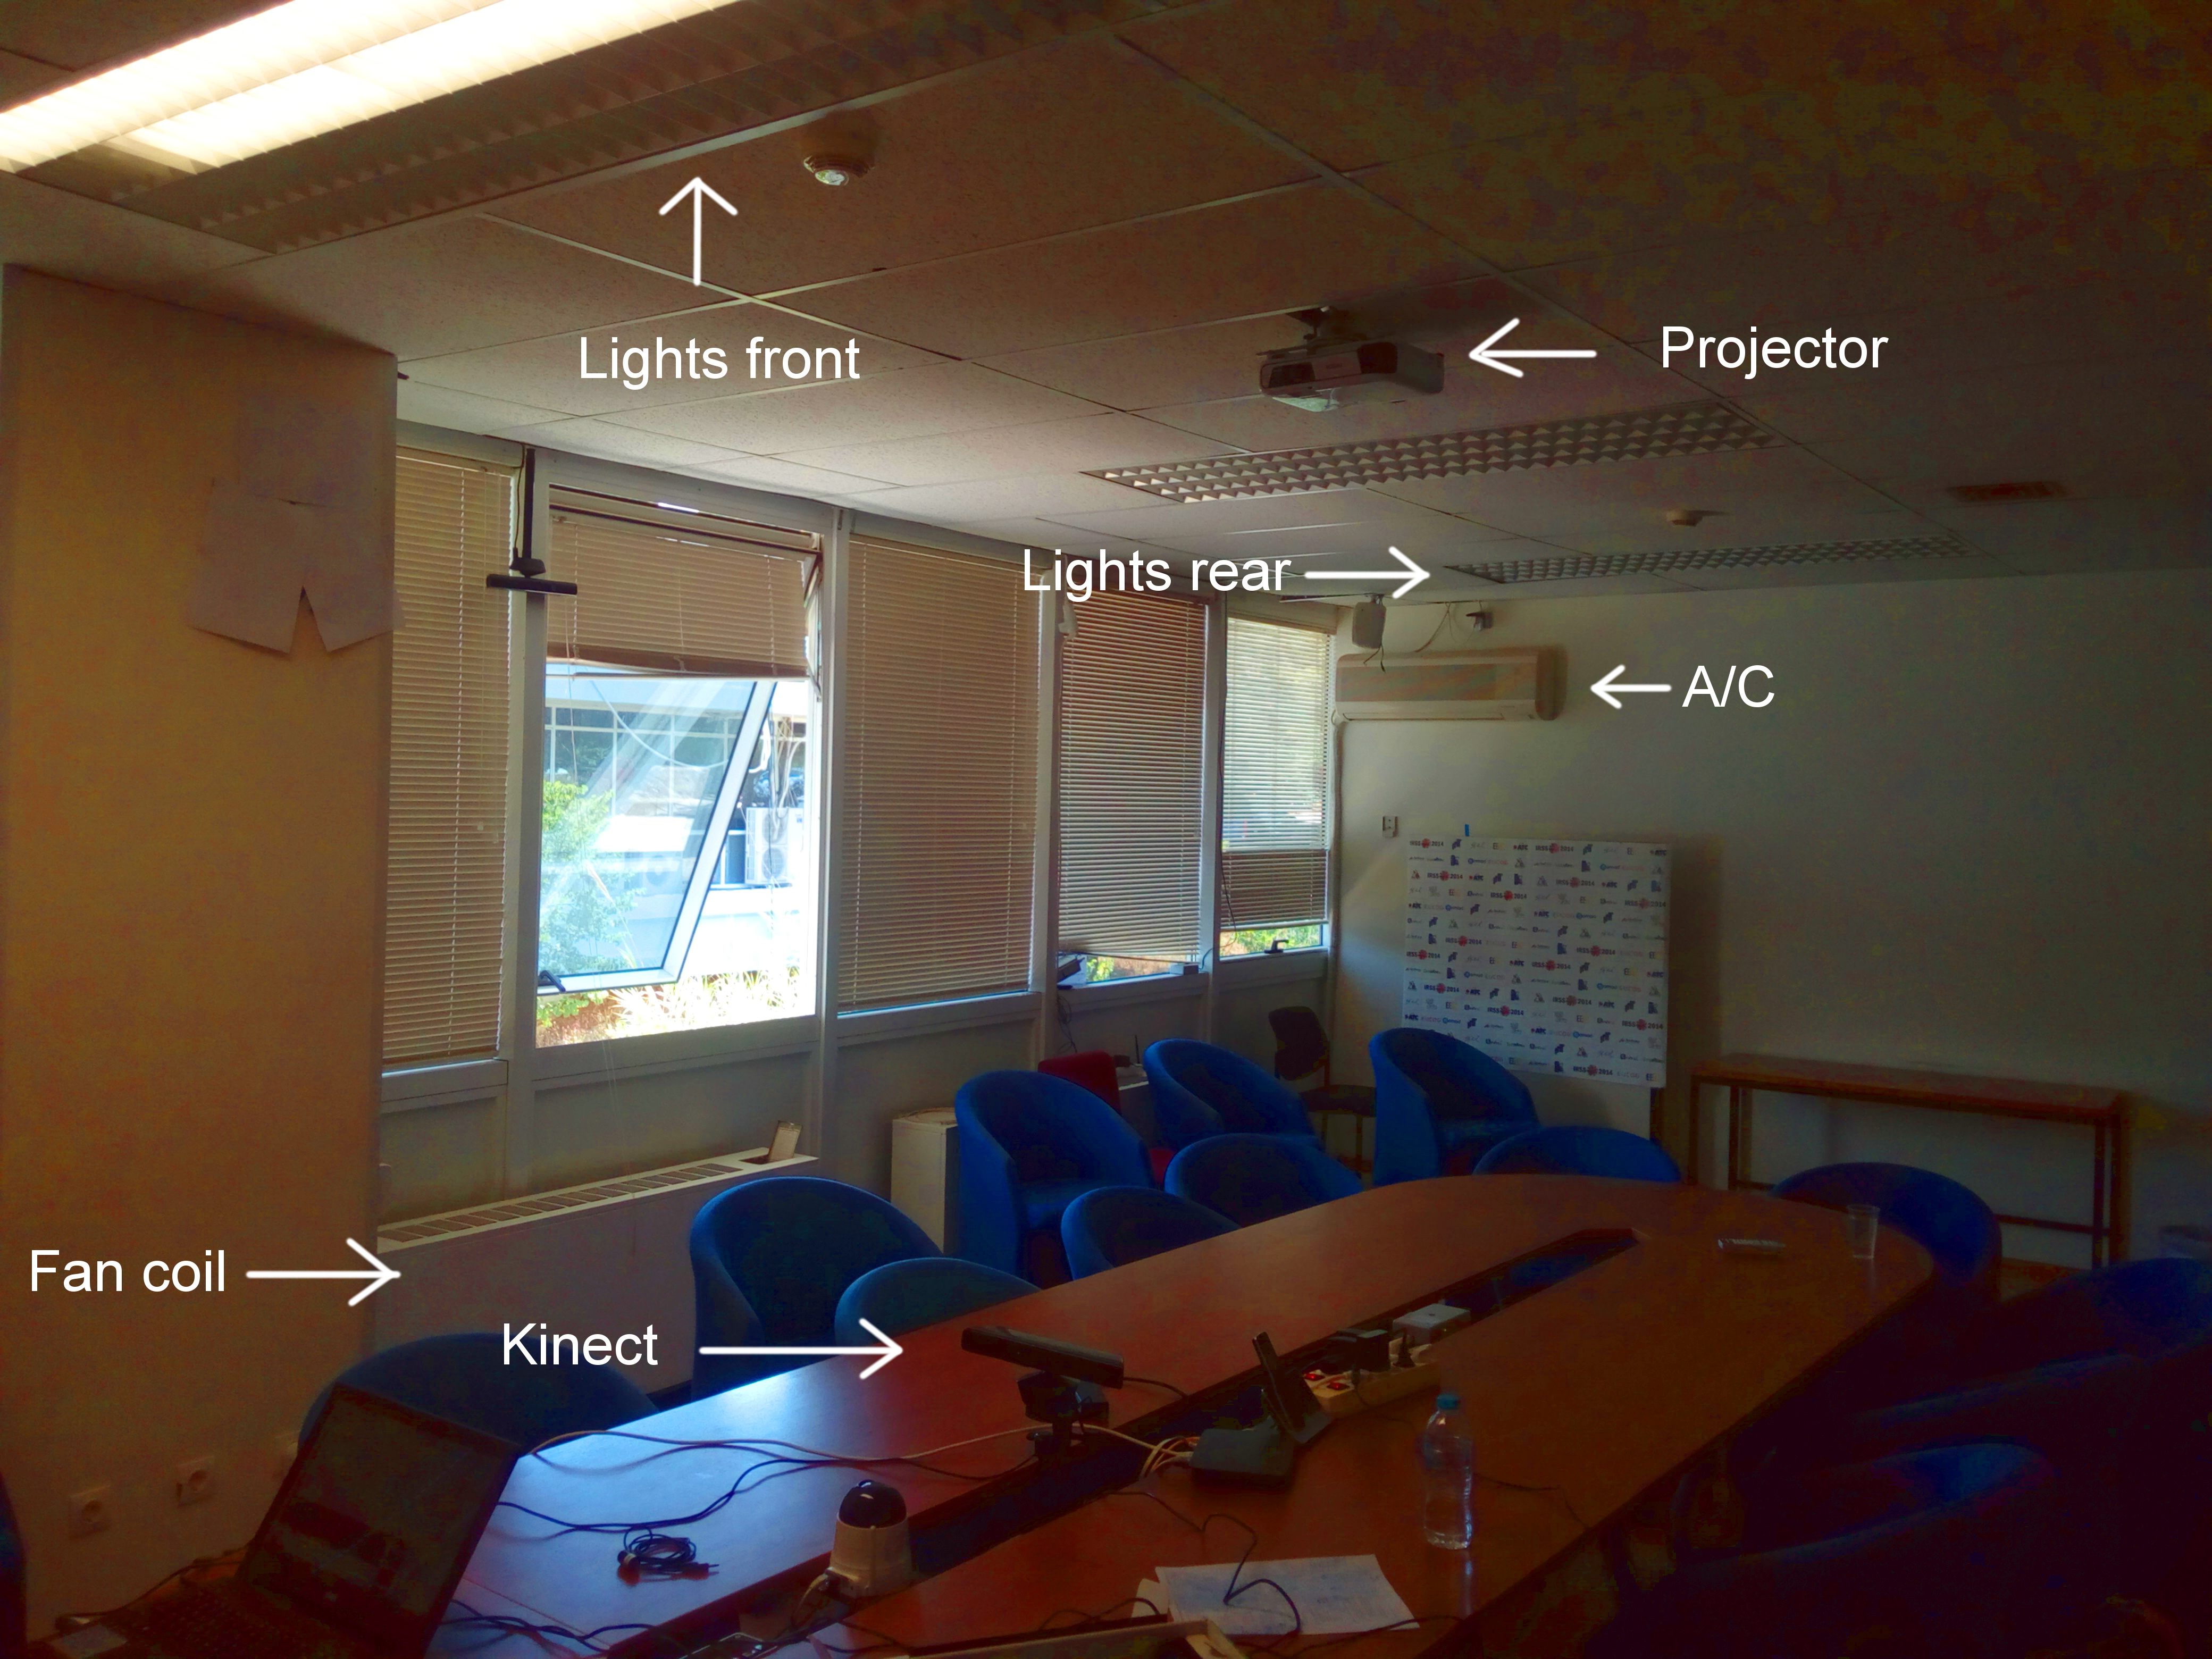
\includegraphics[width=\columnwidth]{figs/aigaio}
\end{figure}
}
\end{frame}

\begin{frame}
\frametitle{Aigaio Devices}

\begin{table}
\centering
\resizebox{0.7\columnwidth}{!}{
\begin{tabular}{l l | l l}
        /pw2                & Projector & /pw3     & Lights Front \\
        /pw4                & A/C       & /pw5     & Fan Coils \\
        /pw6                & Fan Coils & /pw8     & Lights Rear \\
        /ir\_control/action & IR Module &
    \end{tabular}
}
\end{table}

\begin{figure}[ht!]
\centering
\resizebox{\columnwidth}{!}{

\begin{tikzpicture}[sibling distance=9em,
  every node/.style = {shape=rectangle, rounded corners,
    draw, align=center,
    top color=white, bottom color=gray!20}]]
  \node {/demokritos/iit/aigaio} 
    child { node {/ir\_control/action} }
    child { node {/plugwise/action}
    	child { node {/pw2} }
    	child { node {/pw3} }
    	child { node {/pw4} }
    	child { node {/pw5} }
    	child { node {/pw6} }
    	child { node {/pw8} }
  };
\end{tikzpicture}
}
\end{figure}

\end{frame}


\begin{frame}
\frametitle{Aigaio NUI components}
\Wider[5em]{

\begin{figure}[!htb]
\centering
\resizebox{\columnwidth}{!}{
	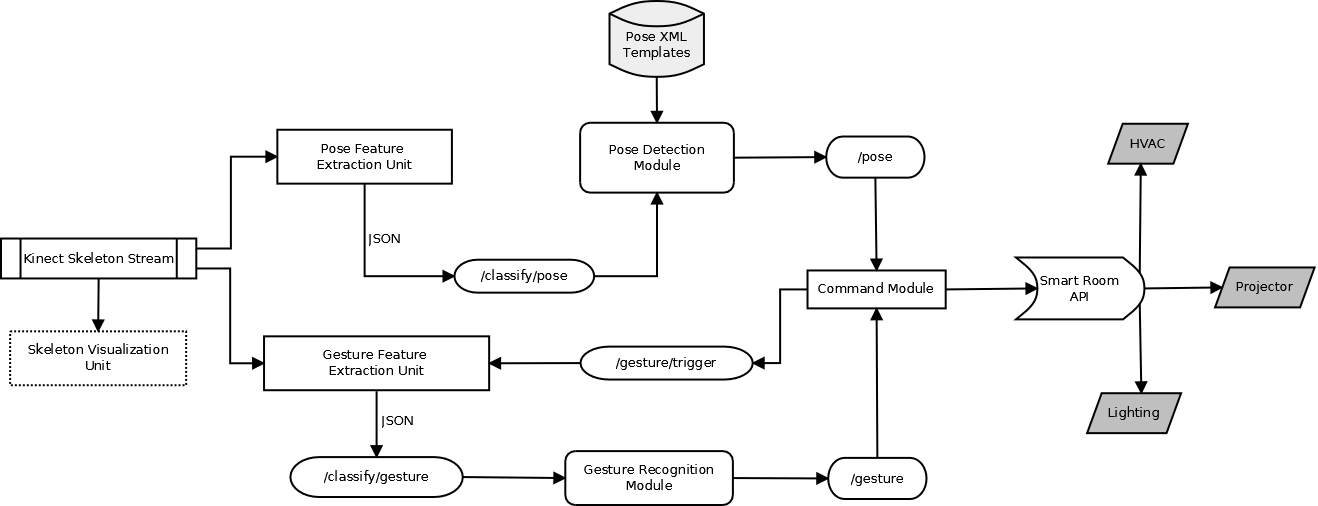
\includegraphics[]{figs/block-diagram}
}
\end{figure}
}

\end{frame}


\begin{frame}
\frametitle{Aigaio NUI services}
\Wider[5em]{

\begin{figure}[!htb]
\centering
\resizebox{\columnwidth}{!}{
	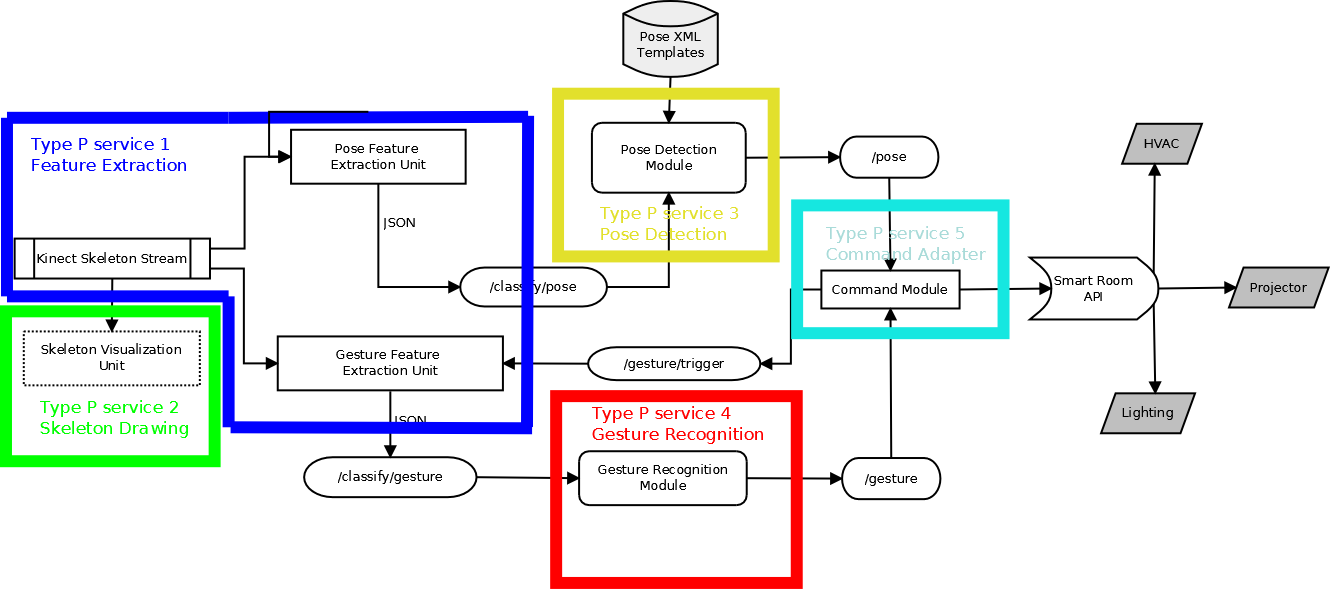
\includegraphics[]{figs/block-diagram-services}
}
\end{figure}
}

\end{frame}


\begin{frame}
\frametitle{Aigaio NUI technology stack}
\Wider[5em]{

\begin{figure}[!htb]
\centering
\resizebox{\columnwidth}{!}{
	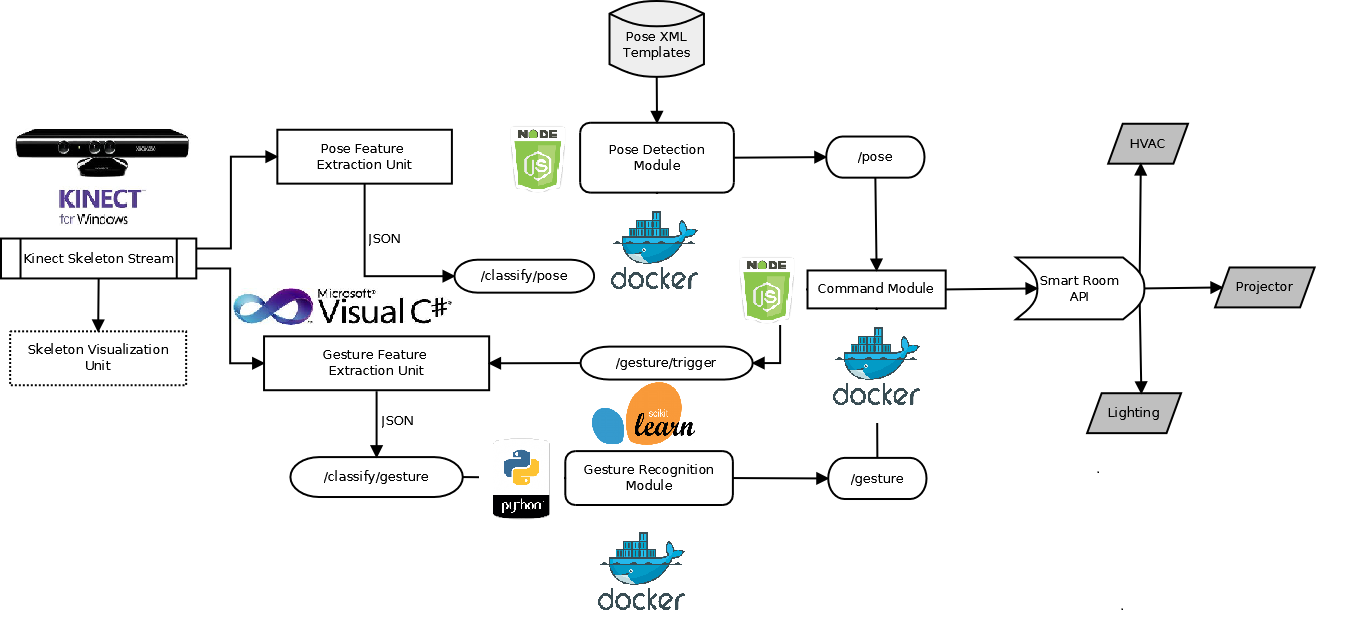
\includegraphics[]{figs/block-diagram-tech}
}
\end{figure}
}
\end{frame}


%!TEX root = main.tex
\section{Conclusions and Future Work}

\begin{frame}
\frametitle{Conclusions}

In this project we have

\begin{itemize}
\item Implemented a simple and efficient \textbf{pose detection} algorithm
\item Constructed a real-time machine learning approach to \textbf{gesture recognition}
\item \textbf{Integrated} these techniques to a real life \textbf{IOT} application for a \textbf{Natural User Interface}
\end{itemize}

\end{frame}

\begin{frame}
\frametitle{Publications}

\begin{itemize}
\item \textbf{G. Paraskevopoulos}, E. Spyrou and D. Sgouropoulos, \textit{A Real-Time Approach for Gesture Recognition using the Kinect Sensor}. In Proc. of Hellenic Conference on Artificial Intelligence (SETN), \textbf{2016}
\item $2$ more upcoming
\end{itemize}

\end{frame}

\begin{frame}
\frametitle{Future Work}

\begin{itemize}
\item Apply the aforementioned techniques to \textbf{new} / \textbf{more challenging} problem domains
\item Construct a \textbf{larger data set} with more users performing a bigger variety of gestures
\item \textbf{Reduce} the \textbf{size/cost} of the needed computing devices
\item Implement a \textbf{dynamic time segmentation} method for gesture detection
\end{itemize}

\end{frame}
\plain{Questions?}
\plain{Thank you!}
%!TEX root = main.tex
\section{Backup Slides}

\begin{frame}
\frametitle{What about Gesture Detection?}

\begin{figure}[!htb]
\centering
\resizebox{\columnwidth}{!}{
	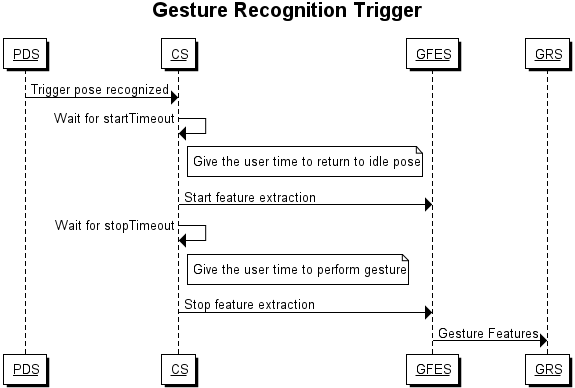
\includegraphics[]{figs/gesturerec-trigger}
}
\end{figure}

\end{frame}

\begin{frame}
\frametitle{Why not a stream of poses?}

$2$ main approaches

\begin{itemize}
\item \textbf{FSM} of intermediate poses: Every new gesture needs to be hard coded
\item \textbf{HMM} with intermediate poses as observations: Generalizes but couples recognition accuracy with frame rate / network stability
\end{itemize}

\end{frame}

\begin{frame}
\frametitle{Kinect on Raspberry Pi}

\textbf{APPROACH}

Use Windows 10 IOT Edition

\textbf{PROBLEMS}

\begin{itemize}
\item Does not support Kinect drivers and Kinect SDK
\item Not enough voltage provided through USB hub to sustain the Kinect sensor
\end{itemize}

\end{frame}



\begin{frame}
\frametitle{Kinect on Raspberry Pi}

\textbf{APPROACH}

\begin{itemize}
\item Use USB over IP to stream the low level Kinect data from a Raspberry Pi 
to a Windows Server so that it appears the Kinect sensor is connected to the server
\item Cross-Compile the Linux kernel with USB-IP modules support
\end{itemize}

\textbf{PROBLEMS}

\begin{itemize}
\item USB-IP modules do not support USB hubs
\item Bandwidth limitations
\end{itemize}

\Wider[5em] {
\begin{figure}[!htb]
\centering
\resizebox{\columnwidth}{!}{
	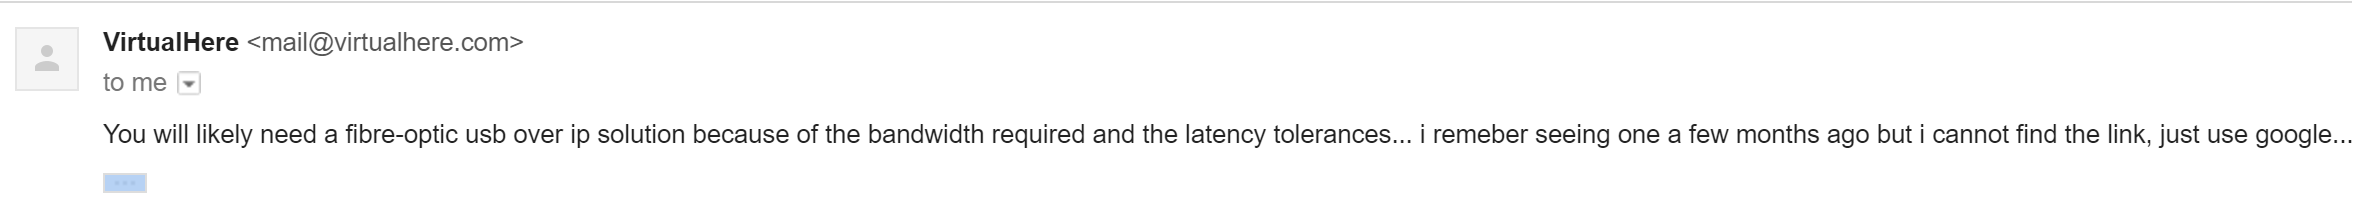
\includegraphics[]{figs/virtualhere-email}
}
\end{figure}
}
\end{frame}

\begin{frame}[fragile]
\frametitle{Why C\#? Why Python? Why JS?}

\textbf{C\#}

\begin{itemize}
\item \texttt{Kinect SDK}
\end{itemize}

\textbf{Python}

\begin{itemize}
\item \texttt{scikit-learn}
\end{itemize}

\textbf{JS}
\begin{itemize}
\item 
\begin{lstlisting}[
    basicstyle=\footnotesize, %or \small or \footnotesize etc.
]
  async.parallel(
    // List of pose detectors to run concurrently
    Object.keys(poseDetectors)
      .reduce((prev, pose) => {
        prev[pose] = poseDetectors[pose](features)
        return prev
      }, {}),
    (err, result) => {
      /* handle list of results ... */
    })
\end{lstlisting}

\end{itemize}

\end{frame}



\appendix

%\begin{frame}[allowframebreaks]
%\frametitle{Bibliography}
%\nocite{*}
%\printbibliography[heading=none]

%\end{frame}

\end{document}